\pagenumbering{arabic}
\section{论文背景}
经典的聚类算法K-means、 K-medoids 通过指定聚类中心,再通过迭代的方式更新聚类中心,由于每个点都被指派到最近的聚类中心,所以导致其无法检测出球形簇。DBSCAN等基于密度的聚类方法可以对于任意形状分布进行聚类,但是必须指定一个密度阈值,从而去除低于此密度阈值的噪音点,而这个密度阈值往往很难确定。

本文提出的基于局部密度峰值的算法则可以解决K-means、 K-medoids的不适用于非球状簇分类的问题。同时,由于本文提出的方法不需要指定类别的数量,所以相对于DBSCAN来讲,本文的方法更加容易进行操作。

\section{核心思想}
聚类中心应该具有两种特点:1.被具有较低局部密度的邻居点包围。   2.与具有更高密度的任何点有相对较大的距离。

我认为可以通过这样的类比来进行理解:每一个蔟就相当于是一座山峰,而聚类中心就是山顶。山顶是被较低海拔的石头包围,而山顶和山顶之间的距离很远。本文的新算法就是基于这两点来识别和查找聚类中心。

下面先介绍该算法的两个重要概念:局部密度和最小距离。接着在此基础上说明改算法的可行性。

\subsection{局部密度}
定义第$i$个元素的局部密度$\rho_i$为
$$ \rho_i=\sum_{j} \chi(d_{ij}-d_c)$$

其中当$x<0$时,$\chi(x)=1$,当$x>=0$时,$\chi(x)=0$,$\d_{ij}$表示第$i$个元素与第$j$个元素的距离,$d_c$表示截断距离。通俗来讲,$\rho_i$就是与其相距距离小于$d_c$的点的个数。


由于局部密度只是一个衡量指标,所以我们也可以使用下述定义来表示第$i$个元素的局部密度(即Gaussian kernel)
$$ \rho_i=\sum_{j} e^{-{(\frac{d_{ij}}{d_c})^2}}$$

由上式可以看出,每个样本点都$\rho_i$有贡献,并且与点$i$的距离越近,其权重就越大。


\subsection{最小距离}
定义$\delta_i$为点$i$到任何比其局部密度大的点的距离的最小值,我们下面简称为最小距离。
$$ \delta_i = \min_{j:\rho_j>\rho_i}{d_{ij}} $$

对于密度最大的点,我们定义其最小距离为
$$ \delta_i = \max_{j}{d_{ij}} $$

\subsection{算法的可行性}
根据上述定义我们可以知道,如过一个点是聚类中心,那么该点的的局部密度$\rho_i$肯定是要高于其周围点的。并且其最小距离$\delta_i$也是比较大的。基于这两个特点,我们将$\rho_i$和$\delta_i$标准化后进行相乘记为$\gamma$,那么该值要远大于非聚类中心点的值。所以我们可以通过该算法找到聚类中心点。

图\ref{Figure_1}为一个数据集的$\delta$-$\rho$图和$\gamma$图,从中我们也可以证实上述说法是正确的。

\begin{figure}[ht]
\centering
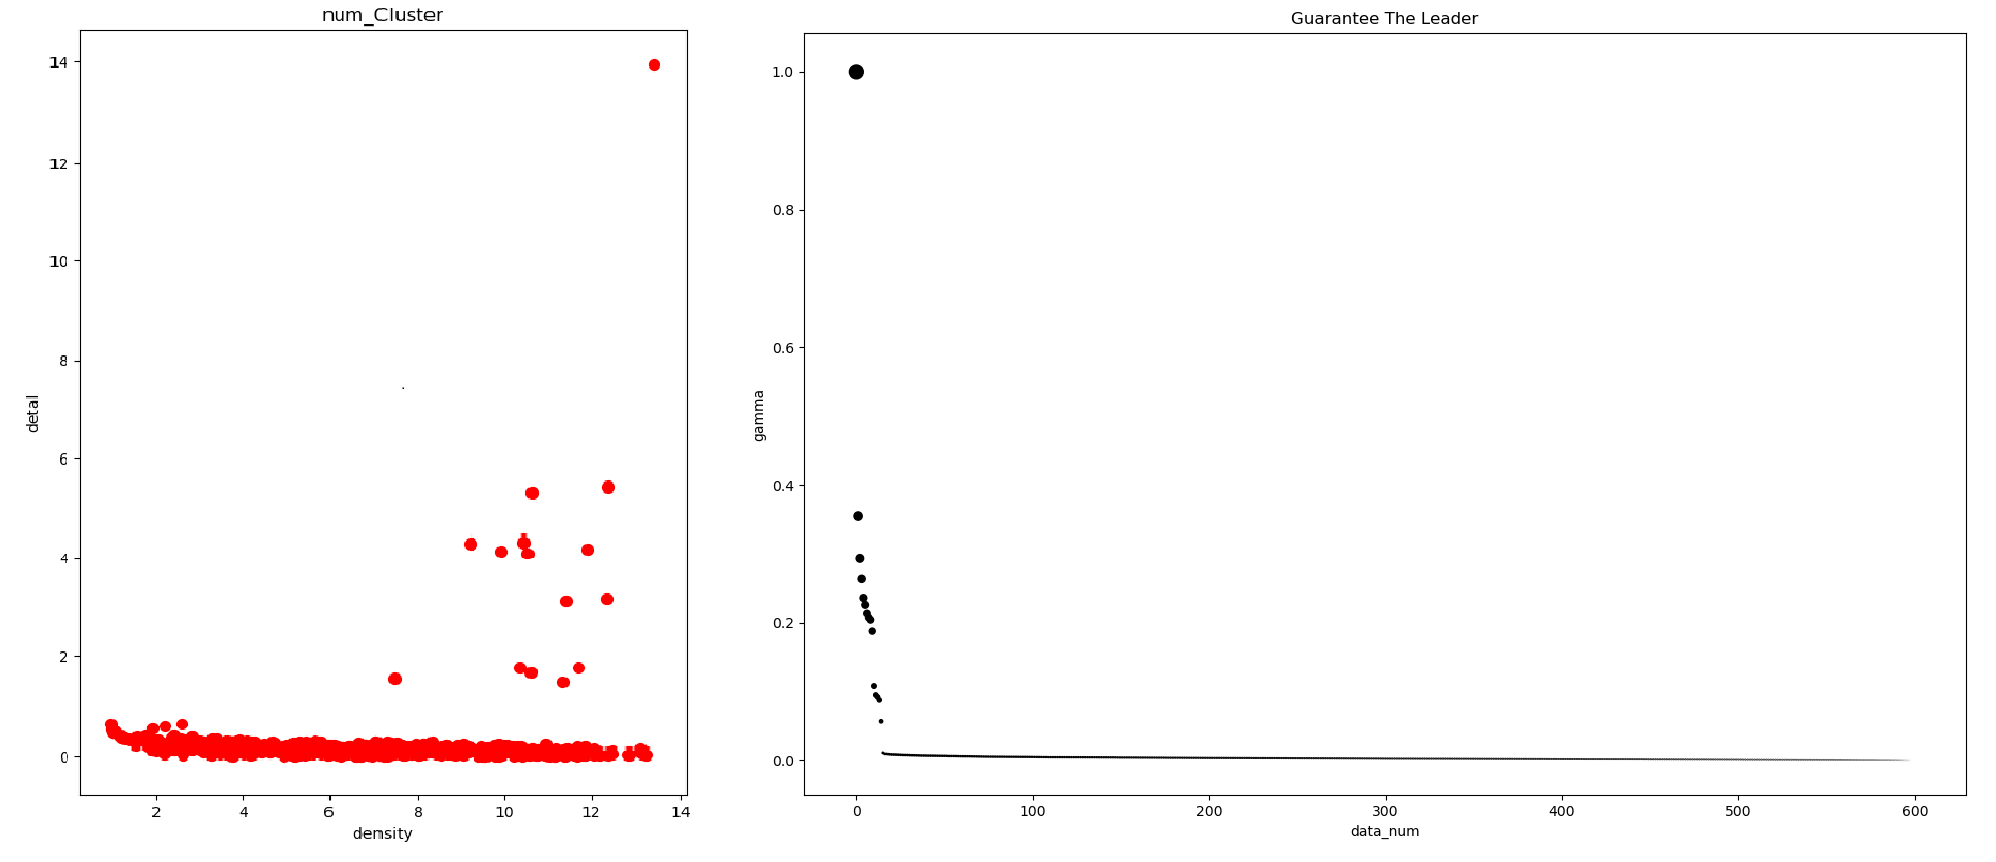
\includegraphics[scale=0.38]{figure/Figure_1.png}%[size][path]
\caption{左图:$\delta$-$\rho$图,横轴为$\rho$,纵轴为$\delta$。\ 右图:$\gamma$图,记录每个点的$\gamma$值}
\label{Figure_1}
\end{figure}

\section{算法原理和步骤}
算法原理可参考上述的算法可行性。下面我们会详细的讲解算法内容。
\subsection{获取距离矩阵}
由论文可知,我们需要的数据基础是所有的点和点之间的距离,所以我们的第一步便是要求出距离矩阵。我在重现论文实验时采用python语言。下面的代码块的功能即是求取距离矩阵。
\begin{lstlisting}[language=python]

def calculate_Distance(data):
    distance_Matrix = np.zeros(shape=(len(data), len(data)))
    for i in range(len(data)):
        for j in range(len(data)):
            if i > j:
                distance_Matrix[i][j] = distance_Matrix[j][i]
            elif i < j:
                distance_Matrix[i][j] = np.sqrt(np.sum(np.power(data[i] - data[j], 2)))
    return distance_Matrix
\end{lstlisting}



\subsection{计算截断距离$dc$}

在获取距离矩阵后,我们需要进行两个最重要的数据的计算:局部密度$\rho$和最小距离$\delta$。由2.1中局部密度$\rho$的定义可以看出,局部密度的计算需要依靠$dc$(截断距离)。所以我们下一步就是获取$dc$。我采用的算法如下:

$dc$为所有点对$(i,j)$距离的前$t\%$。$t$为阈值,可以根据情况自由选择,论文中提到$dc$的取值具有鲁棒性,所以$t$的鲁棒性也是比较好的。$dc$之所以鲁棒性较好,是因为$dc$越大,$\rho$越大,计算$\delta$和选中心点时只比较相对大小,与具体的数值无关。

代码如下:

\begin{lstlisting}[language=python]
def dc_Get(distance_Matrix, tolerance):
    temp_Distance = [] #用于存储所有点对的距离
    for i in range(len(distance_Matrix[0])):
        for j in range(i + 1, len(distance_Matrix[0])):
            temp_Distance.append(distance_Matrix[i][j])
    temp_Distance.sort() #对距离进行升序排序
    dc = temp_Distance[int(len(temp_Distance) * tolerance / 100)] #获取第tolerance%的点对距离作为截断距离
    return dc
\end{lstlisting}


\subsection{获取局部密度$\rho$}
根据上文2.1中可知,我们为局部密度$\rho$提供了两个定义,由于第二个定义(Gaussian kernel)的计算方式涉及到了全体数据,所以我觉得这种方法更加准确些。我写的下列代码提供了两种方法,我把第一个定义的方法给注释了,采用第二种方法。

\begin{lstlisting}[language=python]
def density_Get(distance_Matrix, dc):
    #methon_1
    # density = np.zeros(shape=len(distance_Matrix))
    # for i in range(len(distance_Matrix[0])):
    #     for j in range(len(distance_Matrix[0])):
    #         if distance_Matrix[i][j] <= dc:
    #             density[i] += 1
    # return density
    #methon_2
    density = np.zeros(shape=len(distance_Matrix))
    for index, node in enumerate(distance_Matrix):
        density[index] = np.sum(np.exp(-(node / dc) ** 2))
    return density
\end{lstlisting}


\subsection{获取最小距离$\delta$}
获取最小距离的核心思想,在前面的2.2节中已经介绍。虽然论文中没有提及,但是在代码实现时,我们还需要另外一个量:closest\_Distance,他用于存储比当前点密度高的点集中最近的距离点的索引。我们可以先记住这个量,因为在下面为每个点找归属时会用得到。


\begin{lstlisting}[language=python]
def detal_Get(density, distance_Matrix):
    detal_ls = np.zeros(shape=len(distance_Matrix))#detal_ls存储每个点的detal值
    closest_Distance = np.zeros(shape=len(distance_Matrix), dtype=np.int32)#closest_Distance存储比当前点密度高的点集中最近的距离点的索引
    for index, node in enumerate(distance_Matrix):
        density_Larger_Than_Node = np.squeeze(np.argwhere(density > density[index]))#存储比当前点密度大的点
        if density_Larger_Than_Node.size != 0:#如果有密度大于自己的点
            #所有密度大于自己的点与自己的距离集合(一维数组或者一个数)
            distance_Between_Larger_Node = distance_Matrix[index][density_Larger_Than_Node]
            detal_ls[index] = np.min(distance_Between_Larger_Node)
            min_Distance_Index = np.squeeze(np.argwhere(distance_Between_Larger_Node == detal_ls[index]))
            #存在多个密度大于自己且距离自己最近的点时,选择一个点
            if min_Distance_Index.size >= 2:
                min_Distance_Index = np.random.choice(a=min_Distance_Index)
            if distance_Between_Larger_Node.size > 1:
                closest_Distance[index] = density_Larger_Than_Node[min_Distance_Index]
            else:
                closest_Distance[index] = density_Larger_Than_Node
        #对于最大密度的点
        else:
            detal_ls[index] = np.max(distance_Matrix)
            closest_Distance[index] = index
    return detal_ls, closest_Distance
\end{lstlisting}

\subsection{$\delta$-$\rho$图及$\gamma$(决策)图}
截止到现在为止,我们需要的数据都已经准备好了。前面提到,我们将会根据$\delta\times\rho$来选择聚类的蔟数。在代码实现中,我们首先画出$\delta$-$\rho$图。然后将$\delta$和$\rho$进行标准化后相乘,再画出$\gamma$(决策)图。

在画$\delta$-$\rho$图的过程中,我们顺便画出了原数据散点图,效果见图\ref{figure1_1}。代码如下:
\begin{lstlisting}[language=python]
def show_DensityDetal_And_Dataset(density, detal_Ls, data):
    plt.figure(num=1, figsize=(15, 9))
    #第一个子图为detal-density散点图
    ax1 = plt.subplot(121)
    for i in range(len(data)):
        plt.scatter(x=density[i], y=detal_Ls[i], c='r', marker='o', s=50)
    plt.xlabel('density')
    plt.ylabel('detal')
    plt.title('num_Cluster')
    plt.sca(ax1)
    #第二个子图为原始数据点的散点图
    ax2 = plt.subplot(122)
    for j in range(len(data)):
        plt.scatter(x=data[j, 0], y=data[j, 1], marker='o', c='b', s=50)
    plt.xlabel('axis_x')
    plt.ylabel('axis_y')
    plt.title('set_Data')
    plt.sca(ax2)
    plt.show()
\end{lstlisting}


\begin{figure}[ht]
\centering
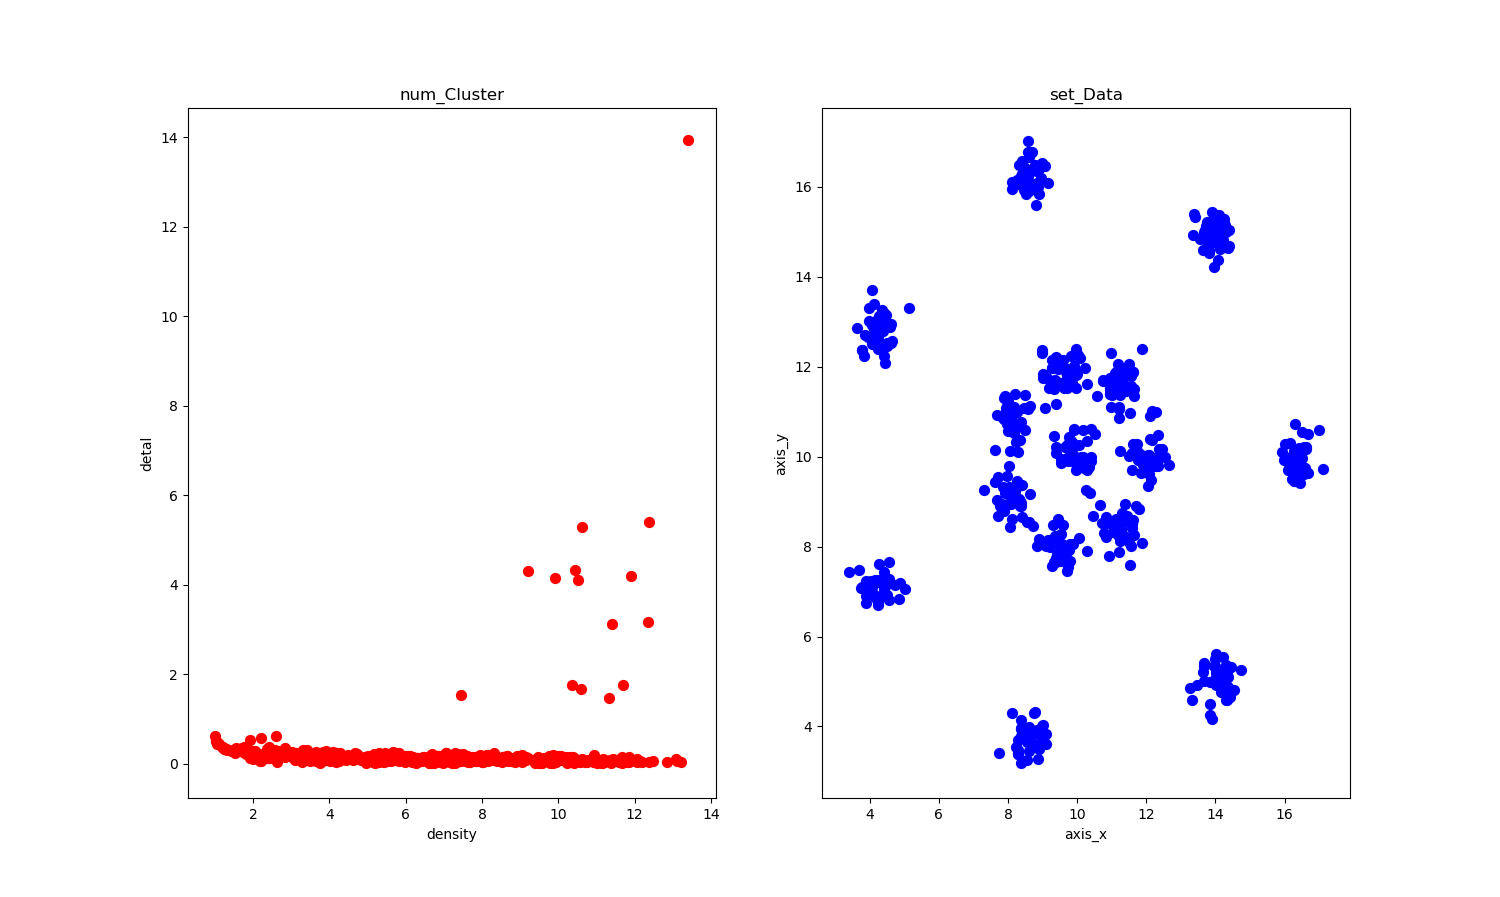
\includegraphics[scale=0.45]{figure/1_1.png}%[size][path]
\caption{左图:$\delta$-$\rho$图,横轴为$\rho$,纵轴为$\delta$。\ 右图:原数据散点图}
\label{figure1_1}
\end{figure}

由图\ref{figure1_1}右图可以看出,该数据集有十五个蔟。由左图可以看出,在左图的右上方也是有十五个点。接着我们用$\gamma$(决策)图来验证一下。


\begin{figure}[ht]
\centering
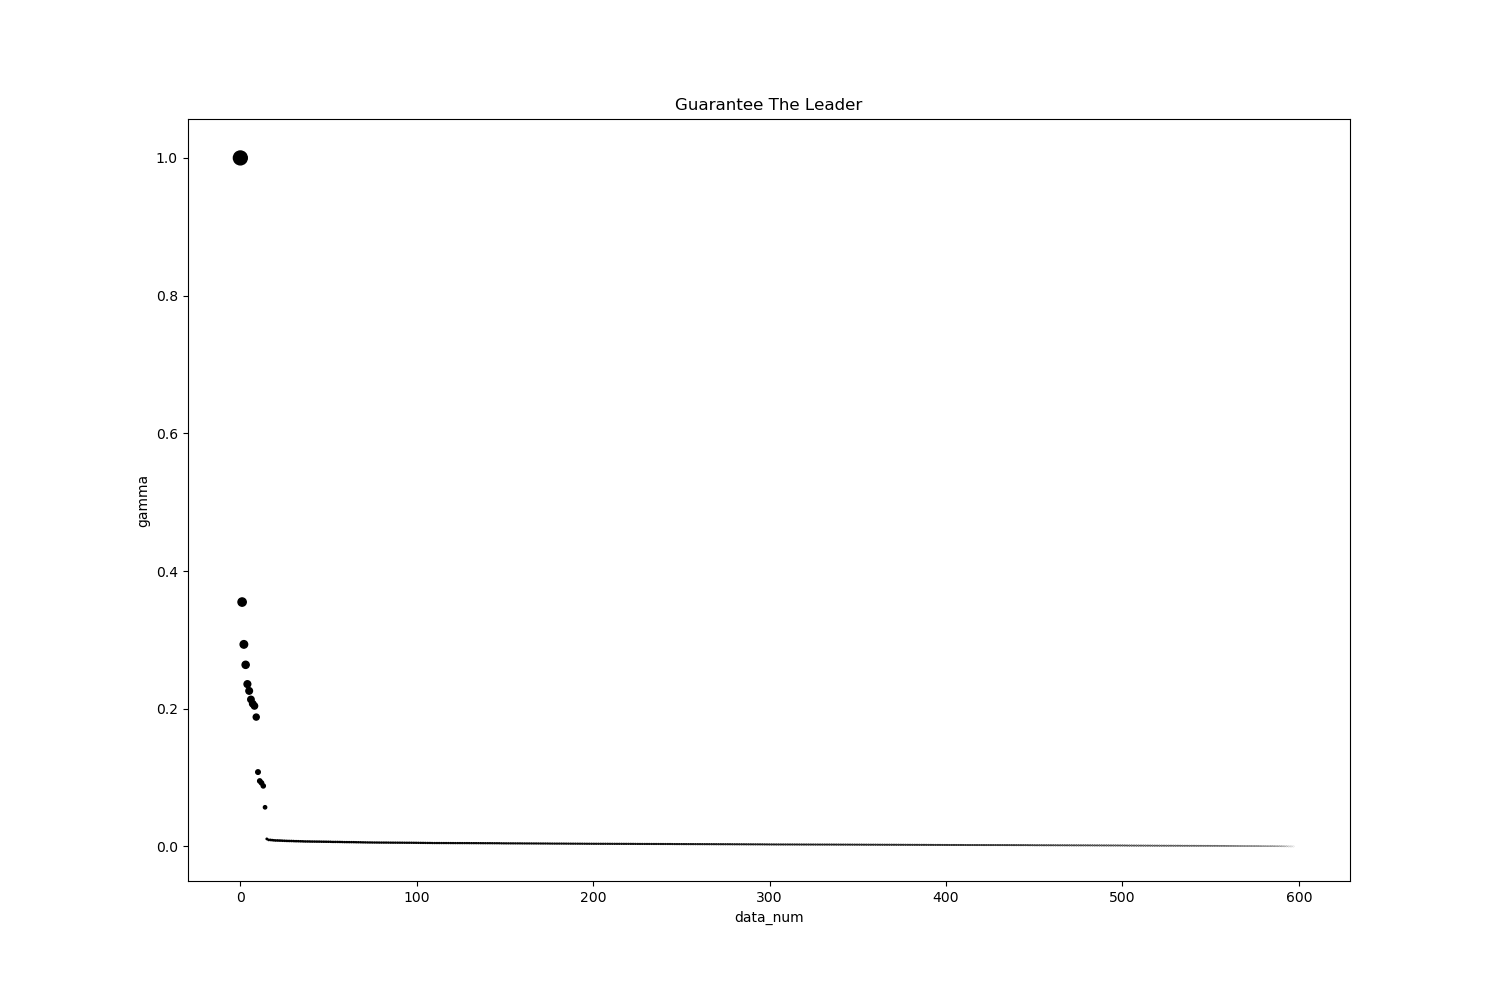
\includegraphics[scale=0.45]{figure/1_2.png}%[size][path]
\caption{$\gamma$(决策)图}
\label{figure1_2}
\end{figure}

$\gamma$(决策)图代码如下:
\begin{lstlisting}[language=python]
def show_Decision_Graph(density, detal_Ls):
    #  由于密度和最短距离两个属性的数量级可能不一样,分别对两者做归一化使结果更平滑
    normal_Density = (density - np.min(density)) / (np.max(density) - np.min(density))
    normal_Detal = (detal_Ls - np.min(detal_Ls)) / (np.max(detal_Ls) - np.min(detal_Ls))
    gamma = normal_Density * normal_Detal
    plt.figure(num=2, figsize=(15, 10))
    plt.scatter(x=range(len(detal_Ls)), y=-np.sort(-gamma), c='k', marker='o', s=-np.sort(-gamma) * 100)
    plt.xlabel('data_num')
    plt.ylabel('gamma')
    plt.title('Guarantee The Leader')
    plt.show()
    return gamma
\end{lstlisting}



由图\ref{figure1_2}也可得出,该数据集的蔟数为15。正如预期的那样,只有具有高局部密度和相对较高的距离的点才是类簇中心。

\subsection{为每个点找到归属}
截止到现在,我们已经找到了类簇中心。那么剩余的点属于哪个蔟呢?这部分论文中并没有介绍,经过查阅相关资料、结合自己的想法,我通过下述算法为每个点找到归属。

前面我们介绍到一个数据量:closest\_Distance,他用于存储比当前点密度高的点集中最近的距离点的索引。我们把所有数据集看成一个森林,每一个蔟看成森林的一棵树。那么可以认为,比当前点密度高的点集中最近的距离点的索引就是其父节点。显然每个蔟的聚类中心就是该树的根节点。并且每个点只有一个父节点。那么根据叶节点依次向上回溯,就可以找到其聚类中心,也即是他的归属蔟。我们前面计算得到的closest\_Distance存储的即是我们刚刚说的“父节点”。

代码如下:
\begin{lstlisting}[language=python]
def clustering(clusters_Num, cluster_Centre_Ls):
    for i in range(len(clusters_Num)):
            while clusters_Num[i] not in cluster_Centre_Ls:
                j = clusters_Num[i]
                clusters_Num[i] = clusters_Num[j]
    cluster_Belong = clusters_Num[:]
    return cluster_Belong  #归属
\end{lstlisting}
\subsection{结果展示}
那么截止到现在,每个点都已找到自己所在的蔟。我们看一下效果,见图\ref{figure1_3}(该部分代码就不再展示,详情见附录)。


\begin{figure}[ht]
\centering
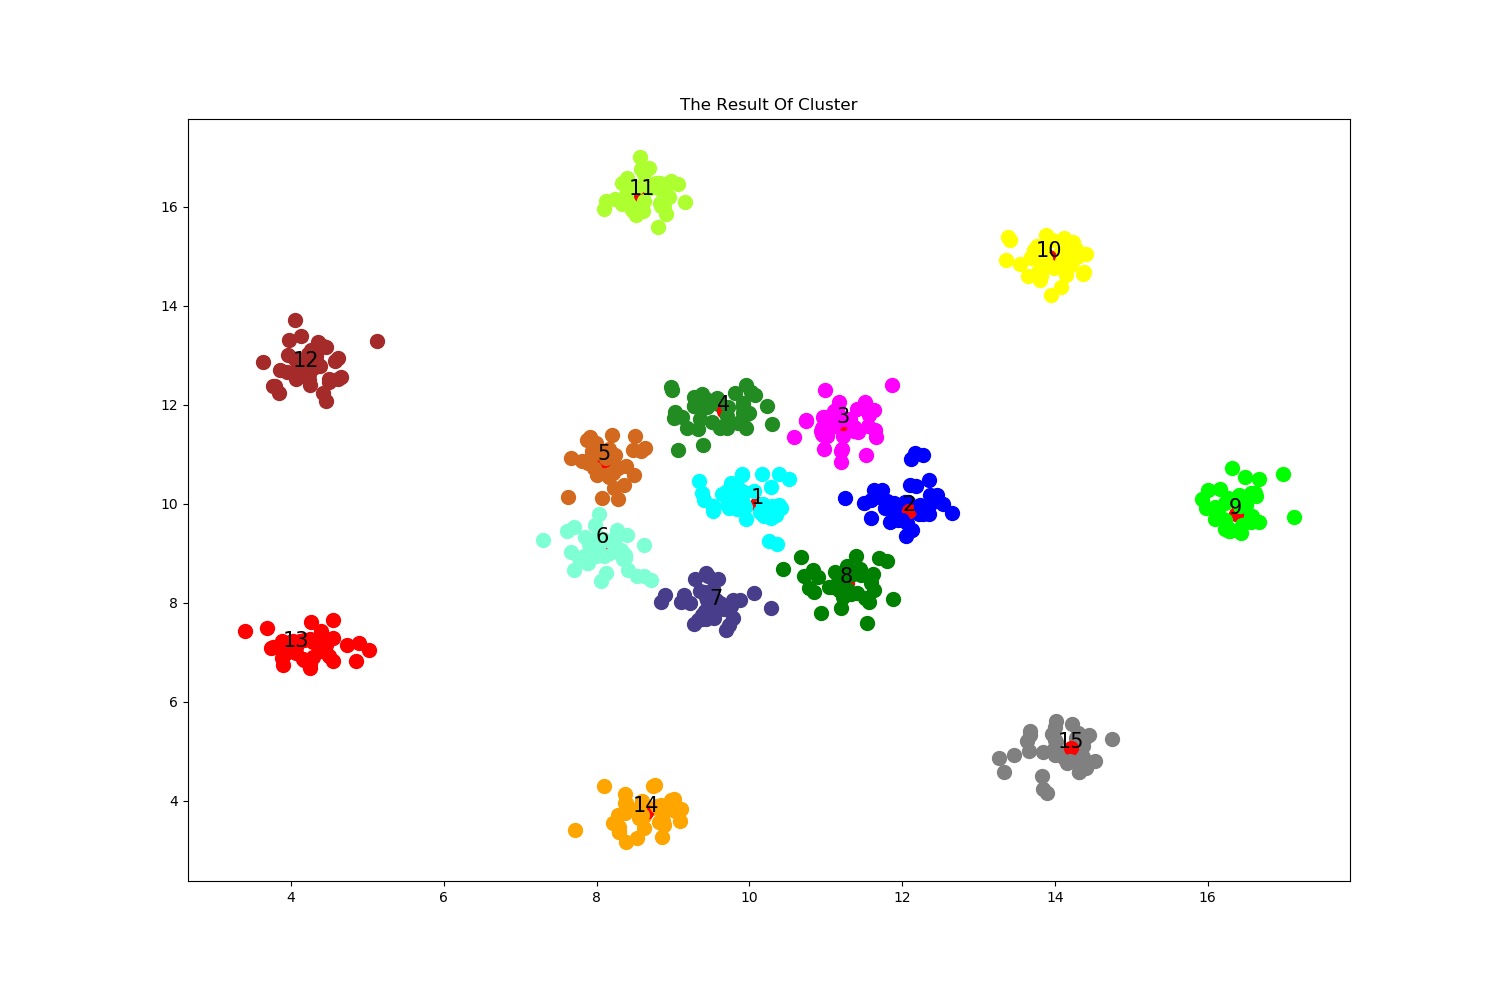
\includegraphics[scale=0.45]{figure/1_3.png}%[size][path]
\caption{结果}
\label{figure1_3}
\end{figure}

\subsection{其他数据集结果展示}
为了说明算法的鲁棒性,我挑选了一些其他类型的数据集进行聚类分析。结果见图\ref{figure2}。由图可以看出应用本算法,这些数据集都能得到不错的效果。

\begin{figure}[ht]
\centering
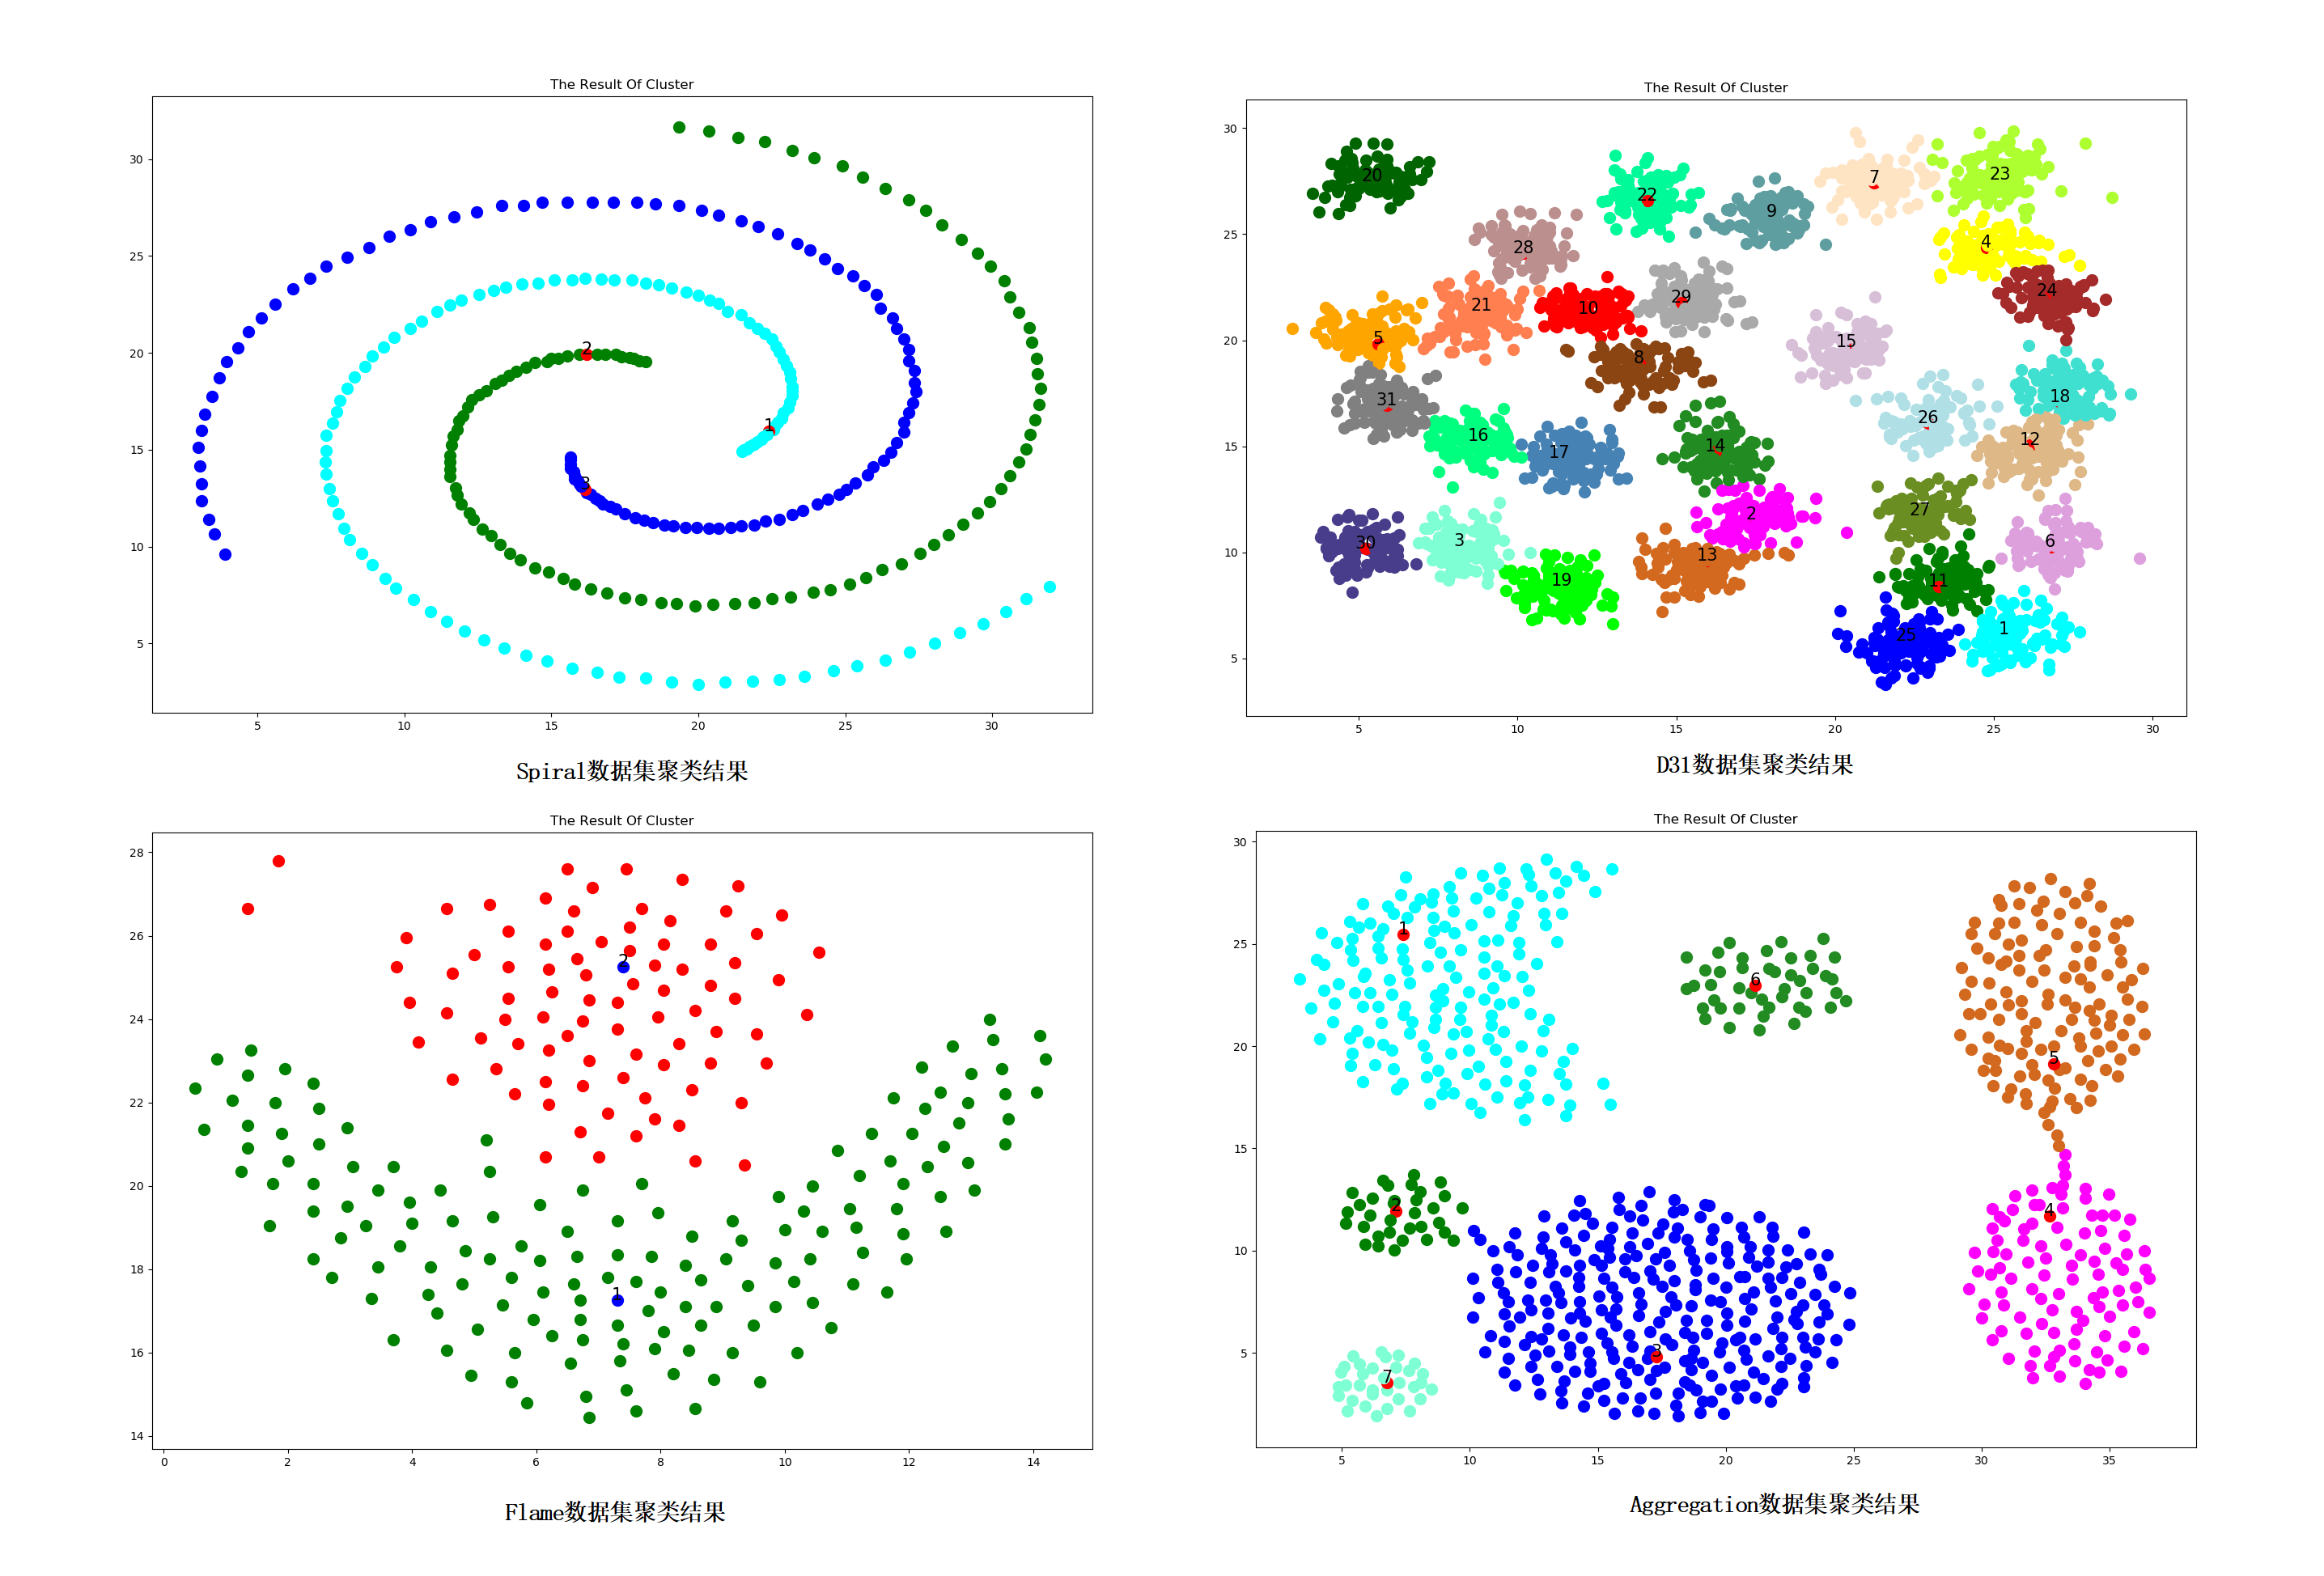
\includegraphics[scale=0.27]{figure/test_2.png}%[size][path]
\caption{}
\label{figure2}
\end{figure}


\section{算法优缺点分析}
\paragraph{算法优点:\\ }


\ \ \  1. 该聚类算法可以得到非球形的聚类结果,可以很好地描述数据分布。

2. 算法复杂度上要比一般的K-means算法的复杂度低,并且不需要迭代。

3. 此算法的只考虑点与点之间的距离,因此不需要将点映射到一个向量空间中。\\

\paragraph{算法缺点:\\ } 


\ \ \  1. 需要事先计算好所有点与点之间的距离。如果样本太大则整个距离矩阵的内存开销特别大,因此如果只需要得到最终聚类中心,则可以考虑牺牲速度的方式计算每一个样本点的和,避免直接加载距离矩阵。

2. 当密度分布不均匀时,效果不好(如Jain数据集)见图\ref{figure2_5},在计算局部密度时并没有考虑局部结构。

3. 应该也不算是缺点吧,毕竟其他方法也没有实现:聚类中心的个数,并不是全自动确定的!!!也是需要人为的对决策图进行判断。
\begin{figure}[ht]
\centering
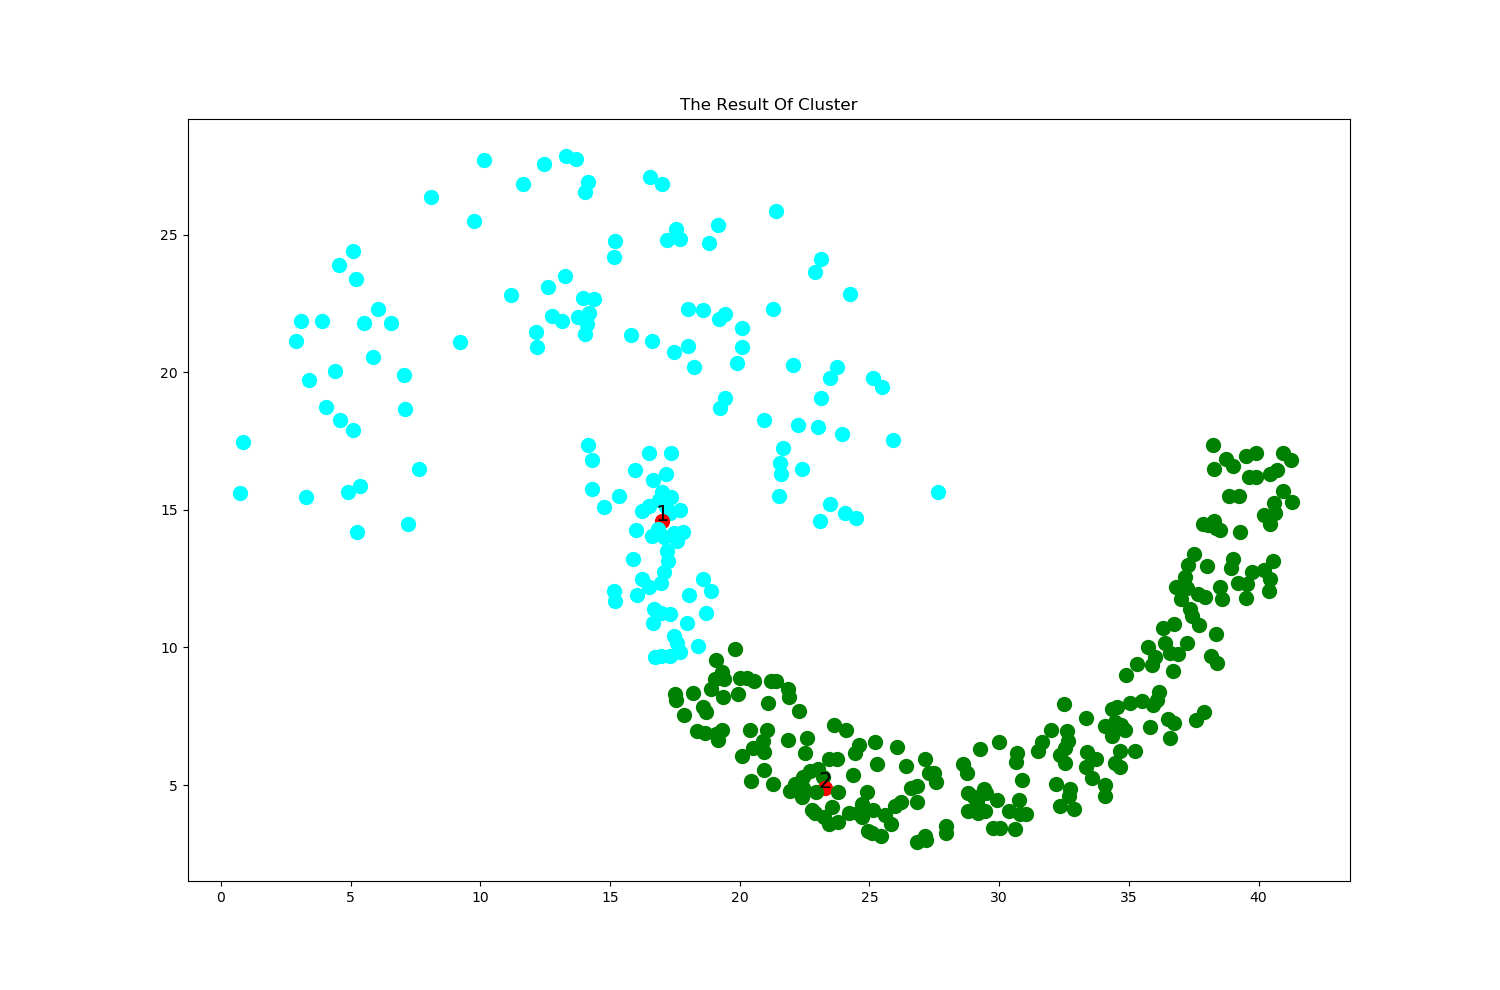
\includegraphics[scale=0.45]{figure/2_5.png}%[size][path]
\caption{Jain数据集聚类结果}
\label{figure2_5}
\end{figure}

\section{总结}

该算法相较于K-means、 K-medoids、DBSCAN等经典算法效果比较好,但是仍然具备一些缺点。比如在图\ref{figure2}右下图Aggregation数据集聚类结果中,如果截断距离$dc$没选择好的话,很有可能会出现右边的两个蔟被聚类成一个蔟的现象(虽然论文说dc的鲁棒性较好),那么这时候聚类的结果可能不如K-means方法。所以从应用的角度来讲,并没有说那个算法一定是强于其他算法的,可能他们针对的问题不同,适用范围不同。所以我觉得合适的算法才是最好的算法。





































